\subsection{Positionnement relatif de n\oe uds}
\label{lib-pos}

\maboite{\BS{usetikzlibrary}\AC{positioning}}


\begin{center}
\RRR{17-5-3}
\end{center}

\begin{tabular}{|c|c|c|}  \hline 
\multicolumn{2}{|c|}{\BS{node} (a) at (1,0) [above=.4cm+.6cm,draw] \AC{XXX};} &  \\ \hline 
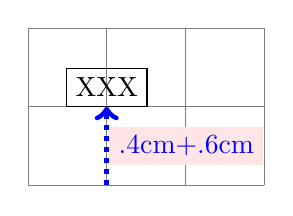
\begin{tikzpicture}
\draw[help lines] (0,0) grid (3,2);
\node (a) at (1,0) [above=.4cm+.6cm,draw] {XXX};
\draw[->,blue,line width=2pt,dotted] (1,0) -- (a.south) node [midway,right,draw=none,fill=red!10] {.4cm+.6cm} ;
\end{tikzpicture} 
&
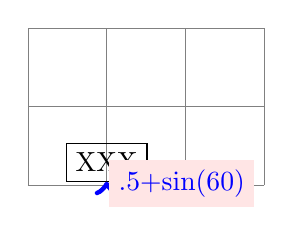
\begin{tikzpicture}
\draw[help lines] (0,0) grid (3,2);
\node (a) at (1,0) [above=.5+sin(60),draw] {XXX};
\draw[->,blue,line width=2pt,dotted] (1,0) -- (a.south) node [midway,right,draw=none,fill=red!10] {.5+sin(60)} ;
\end{tikzpicture}  
&
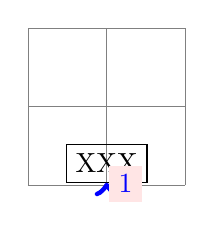
\begin{tikzpicture}
\draw[help lines] (0,0) grid (2,2);
\node (a) at (1,0) [above=1,draw] {XXX};
\draw[->,blue,line width=2pt,dotted] (1,0) -- (a.south) node [midway,right,draw=none,fill=red!10] {1} ;
\end{tikzpicture}  
\\ \hline 
above = \rouge{0.4cm+0.6cm} & above = \rouge{.5+sin(60)}  & above = \rouge{1} \\ 
\hline 
\end{tabular} 

\bigskip

\begin{tabular}{|c|c|} \hline 
\multicolumn{2}{|c|}{\BS{node} (a) at (1,0) [\rouge{above right=3cm and 2cm},draw] \AC{XXX};} \\  \hline 
\begin{tikzpicture}
\draw[help lines] (0,0) grid (5,5);
\node (a) at (1,1) [above right=3cm and 2cm,draw] {XXX};
\draw[->,blue,line width=2pt,dotted] (1,1) |- (a.south west);
\end{tikzpicture}
&  
\begin{tikzpicture}
\draw[help lines] (0,0) grid (5,5);

\node (b) at (1,4) [below right=3cm and 2cm,draw] {XXX};
\draw[->,blue,line width=2pt,dotted] (1,4) |- (b.north west);
\end{tikzpicture}
\\ \hline 
\rouge{above right=3cm and 2cm} & \rouge{below right=3cm and 2cm}
\\ \hline 
\end{tabular}  

\bigskip
 
\begin{tabular}{|c|c|}  \hline 
\begin{tikzpicture}[every node/.style=draw,baseline=1.5cm]
\draw[help lines] (0,0) grid (5,4);
\node (a) at (1,1) {node a};
\node (b) [above=2cm of a.north east] {XXX};
\draw[->,blue,line width=2pt,dotted] (a.north) -- (b.south) node [midway,right,draw=none,fill=red!10] {2cm of a.north east} ;
\end{tikzpicture}
&  
\parbox{8cm}{
\BS{node} (a) at (1,1) \AC{node a}; \\
\BS{node} (b) [\rouge{above=2cm of a.north east}] \AC{XXX};}
\\ \hline 
\end{tabular} 

\bigskip

\begin{tabular}{|c|c|}  \hline 
\begin{tikzpicture}[every node/.style=draw]
\draw[help lines] (0,0) grid (2,3);
\node (a) at (1,0) {node a};
\node (b) [above=1cm of a] {node b};
\node (c) [above=1cm of b] {node c};
\draw[->,blue,line width=2pt,dotted] (a.north) -- (b.south) node [midway,right,draw=none,fill=red!10] {1cm} ;
\draw[->,blue,line width=2pt,dotted] (b.north) -- (c.south) node [midway,right,draw=none,fill=red!10] {1cm} ;
\end{tikzpicture}
&  
\begin{tikzpicture}[every node/.style=draw]
\draw[help lines] (0,0) grid (2,3);
\node (a) at (1,0) {node a };
\node (b) [on grid,above=1cm of a] {node b};
\node (c) [on grid,above=1cm of b] {node c};
\draw[->,blue,line width=2pt,dotted] (a.center) -- (b.center) node [midway,right,draw=none,fill=red!10] {1cm} ;
\draw[->,blue,line width=2pt,dotted] (b.center) -- (c.center) node [midway,right,draw=none,fill=red!10] {1cm} ;
\end{tikzpicture}
\\  \hline 
\BS{node} (a) at (1,0) \AC{node a};  &\BS{node} (a) at (1,0) \AC{node a};   \\ 
\BS{node} (b) [above=1cm of a] \AC{node b};  &\BS{node} (b) [\RDD{on grid},above=1cm of a] \AC{node b};   \\ 
\BS{node} (c) [above=1cm of b] \AC{node c};  &\BS{node} (c) [\RDD{on grid},above=1cm of b] \AC{node c};   \\ 
\hline 
\end{tabular} 

\begin{tabular}{|c|c|} \hline 
\begin{tikzpicture}[every node/.style=draw,node distance=1cm,baseline = 1.5cm]
\draw[help lines] (0,0) grid (2,3);
\node (a1) at (1,0) {node a};
\node (b) [above=of a] {node b};
\node (c) [above=of b] {node c};
\draw[->,blue,line width=2pt,dotted] (a.north) -- (b.south) node [midway,right,draw=none,fill=red!10] {1cm} ;
\draw[->,blue,line width=2pt,dotted] (b.north) -- (c.south) node [midway,right,draw=none,fill=red!10] {1cm} ;
\end{tikzpicture}
 & 
 \parbox{12cm}{ 
\BS{begin}\AC{tikzpicture}[every node/.style=draw,\RDD{node distance}=1mm] \\
\BS{node} (a1) at (1,0) \AC{node a}; \\
\BS{node} (b) [above=of a] \AC{node b}; \\
\BS{node} (c) [above=of b] \AC{node c}; \\
\BS{end}\AC{tikzpicture}
} 
 \\ 
\hline 
\end{tabular} 

\bigskip

\begin{tabular}{|l|l|} \hline 
\begin{tikzpicture}[node distance=2cm]
\draw[help lines] (0,-1) grid (6,1);
\huge
\node[draw] (X) at (0,0) {X};
\node[draw] (a) [right=of X] {a};
\node[draw] (y) [right=of a] {y};
\draw[->,blue,line width=2pt,dotted] (X.east) -- (a.west) node [midway,draw=none,fill=red!10] {\small{2cm}} ;
\draw[->,blue,line width=2pt,dotted] (a.east) -- (y.west) node [midway,draw=none,fill=red!10] {\small{2cm}} ;
\end{tikzpicture}
&  
\begin{tikzpicture}[node distance=2cm]
\draw[help lines] (0,-1) grid (6,1);
\huge
\node[draw] (X) at (0,0) {X};
\node[draw] (a) [base right=of X] {a};
\node[draw] (y) [base right=of a] {y};
\draw[->,blue,line width=2pt,dotted] (X.base east) -- (a.base west) node [midway,draw=none,fill=red!10] {\small{2cm}} ;
\draw[->,blue,line width=2pt,dotted] (a.base east) -- (y.base west) node [midway,draw=none,fill=red!10] {\small{2cm}} ;
\end{tikzpicture}
\\ \hline 
\BS{node}[draw] (X) at (0,0) \AC{X};
&  
\BS{node}[draw] (X) at (0,0) \AC{X};
\\
\BS{node}[draw] (a) [right=of X] \AC{a};
&
\BS{node}[draw] (a) [base right=of X] \AC{a};
\\
\BS{node}[draw] (y) [right=of a] \AC{y};
&
\BS{node}[draw] (y) [base right=of a] \AC{y};
\\ \hline 
\end{tabular} 

